\documentclass[12pt]{article}

\usepackage[a4paper, left=3cm, right=2.5cm]{geometry}
\usepackage[utf8]{inputenc}
\usepackage[english]{babel}
\usepackage{subfigure}
\usepackage{blindtext}
\usepackage{microtype}
\usepackage{graphicx}
\usepackage{float}
\usepackage{wrapfig}
\usepackage{amsmath}
\usepackage[absolute]{textpos}
\usepackage{calc}
\usepackage{hyperref}
\usepackage{listings}
\usepackage{csquotes}

\setcounter{secnumdepth}{4}
\renewcommand{\baselinestretch}{1.2}


\author{Christoph Prenissl}
\date{\today}

\begin{document}

\begin{titlepage}

      \begin{textblock*}{200mm}(4mm, 10mm)
            \begin{figure}
                  \def\svgscale{0.6}
                  \input{oth_logo.pdf_tex}
            \end{figure}
      \end{textblock*}

      \begin{textblock*}{200mm}(96mm, 10mm)
            \begin{tabular}[h]{lr}
                  \textbf{Name:}       & Christoph Prenissl                                                                              \\
                  \textbf{Email:}      & \href{mailto:christoph.prenissl@st.oth-regensburg.de}{christoph.prenissl@st.oth-regensburg.de}\ \\
                  \textbf{Student ID:} & 3174997                                                                                         \\
            \end{tabular}
      \end{textblock*}

      \begin{flushright}
            \today
      \end{flushright}

      \vspace{2cm}

      \begin{center}
            \textbf{\Large{IMDB Software to fetch data of Hollywood Actors and Actresses}}

            \vspace{6cm}

            \textbf{Task 4 - Project Report}

            \vspace{10cm}
      \end{center}
\end{titlepage}

\newpage

\tableofcontents

\newpage

\section{Project Description}
This project mainly consists of creating a Python client to fetch data of the 
\textit{IMDB Top 50 Actors and Actresseslist} and also gather their movie data. 
The client uses an API to fetch all the basic actors/actresses list (\ref{list-actors}),
the actor/actress About section (\ref{about}) and all their movies (\ref{movies}).
For Sections \ref{awards} - \ref{top-movies} Web-scraping is used to 
get awards data and ratings of the movies.
The client is presented in a window based UserInterface where the user 
can click to gather the wanted information.

The specifics are handled in this document.

\section{Tools, Modules and Data-Structure}
\subsection{Presentation Tools}
For presenting the project I also used VS Code. I wrote the reports in \textit{\LaTeX} with the help of the \textit{LaTex Workshop} extension and 
\textit{PlantUml} to present core structures and flows of the client.
In the presentation of the client I used \textit{Powerpoint}. 

\subsection{Development Tools}
For development of the client I used \textit{Python 3.9.4} in \textit{Visual Studio 
Code} with the \textit{Python IntelliSense} extension which helped me in code 
completion and understanding the structure of all the frameworks and modules. For 
version control I used \textit{Git} and the helpful VS Code extension 
\textit{GitLens} which helped me to keep track of my changes in the project files.

The UI was designed with \textit{Qt Designer}. It was very convenient to
have a graphical UserInterface to drag and drop widgets and have an overal 
understanding of all elements.

\subsection{Modules}
When it comes to the modules, \textit{Requests} and \textit{BeautifulSoup 4} were  
necessary to handle all the web scraping. The http context is created with the 
module \textit{SSL}. For most data I used a data frame created with \textit{Pandas}.

The Graphical UserInterface was implemented using \textit{PyQt6}. The framework also
provides Thread libraries to help with multi-threading.

\section{Design}
The client has one base module at the root of the project and the children modules 
\textit{landing} and \textit{detail}.

\begin{figure}[H]
      \begin{center}
            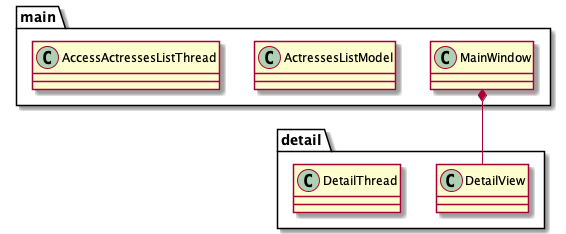
\includegraphics[scale=0.32]{img/class_diagram.png}
            \caption{\label{fig:packages} All packages used in the project with
                  the most important classes.}
      \end{center}
\end{figure}

While the base module only contains the entry point in the \textit{main.py} file,

the \textit{landing} module handles the asynchronous fetching of the actresses 
list (\ref{list-actors}), visualisation and interaction with the list and initializes an DetailView 
from \textit{detail} when a list element gets accessed.
\textit{MainWindow} is a QObject class which handles the UI update and communicates with 
\textit{AccessActressesListThread} for data provision. For the ListView containing the actresses/actors 
in MainWindow \textit{ActressesListModel} is used for correctly displaying the actor/actress data.
\textit{ActressListElement} is a data wrapper for all the data to present in the list.

The \textit{detail} module helds logic for fetching deeper information with multi-threading on 
an actor or actress regarding ratings and awards. It also contains the code for UI displaying and 
updates.
The \textit{DetailView} class acts analogously to MainView as an controller for handling UI updates and
triggering events on its threads. These threads manage the workers \textit{MoviesDataWorker} and 
\textit{ActressAwardDataWorker} for retrieving the needed data. \textit{ActressDetail} functions as a 
wrapper for a data instance.

\newpage

\section{Functionalities}
In this section all the necessary specifications for the project will be further discussed.

\subsection{List of all available actors and actresses} \label{list-actors}
\begin{figure}[h]
      \centering
      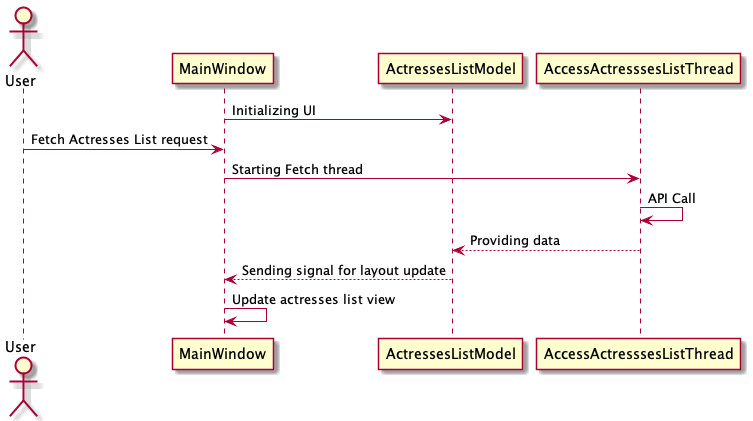
\includegraphics[width=0.45\textwidth]{img/fetch_actresses_flow.png}
      \caption[width=0.45\textwidth]{\label{fig:fetch-actresses-flow} Main flow of fetching actresses list}
      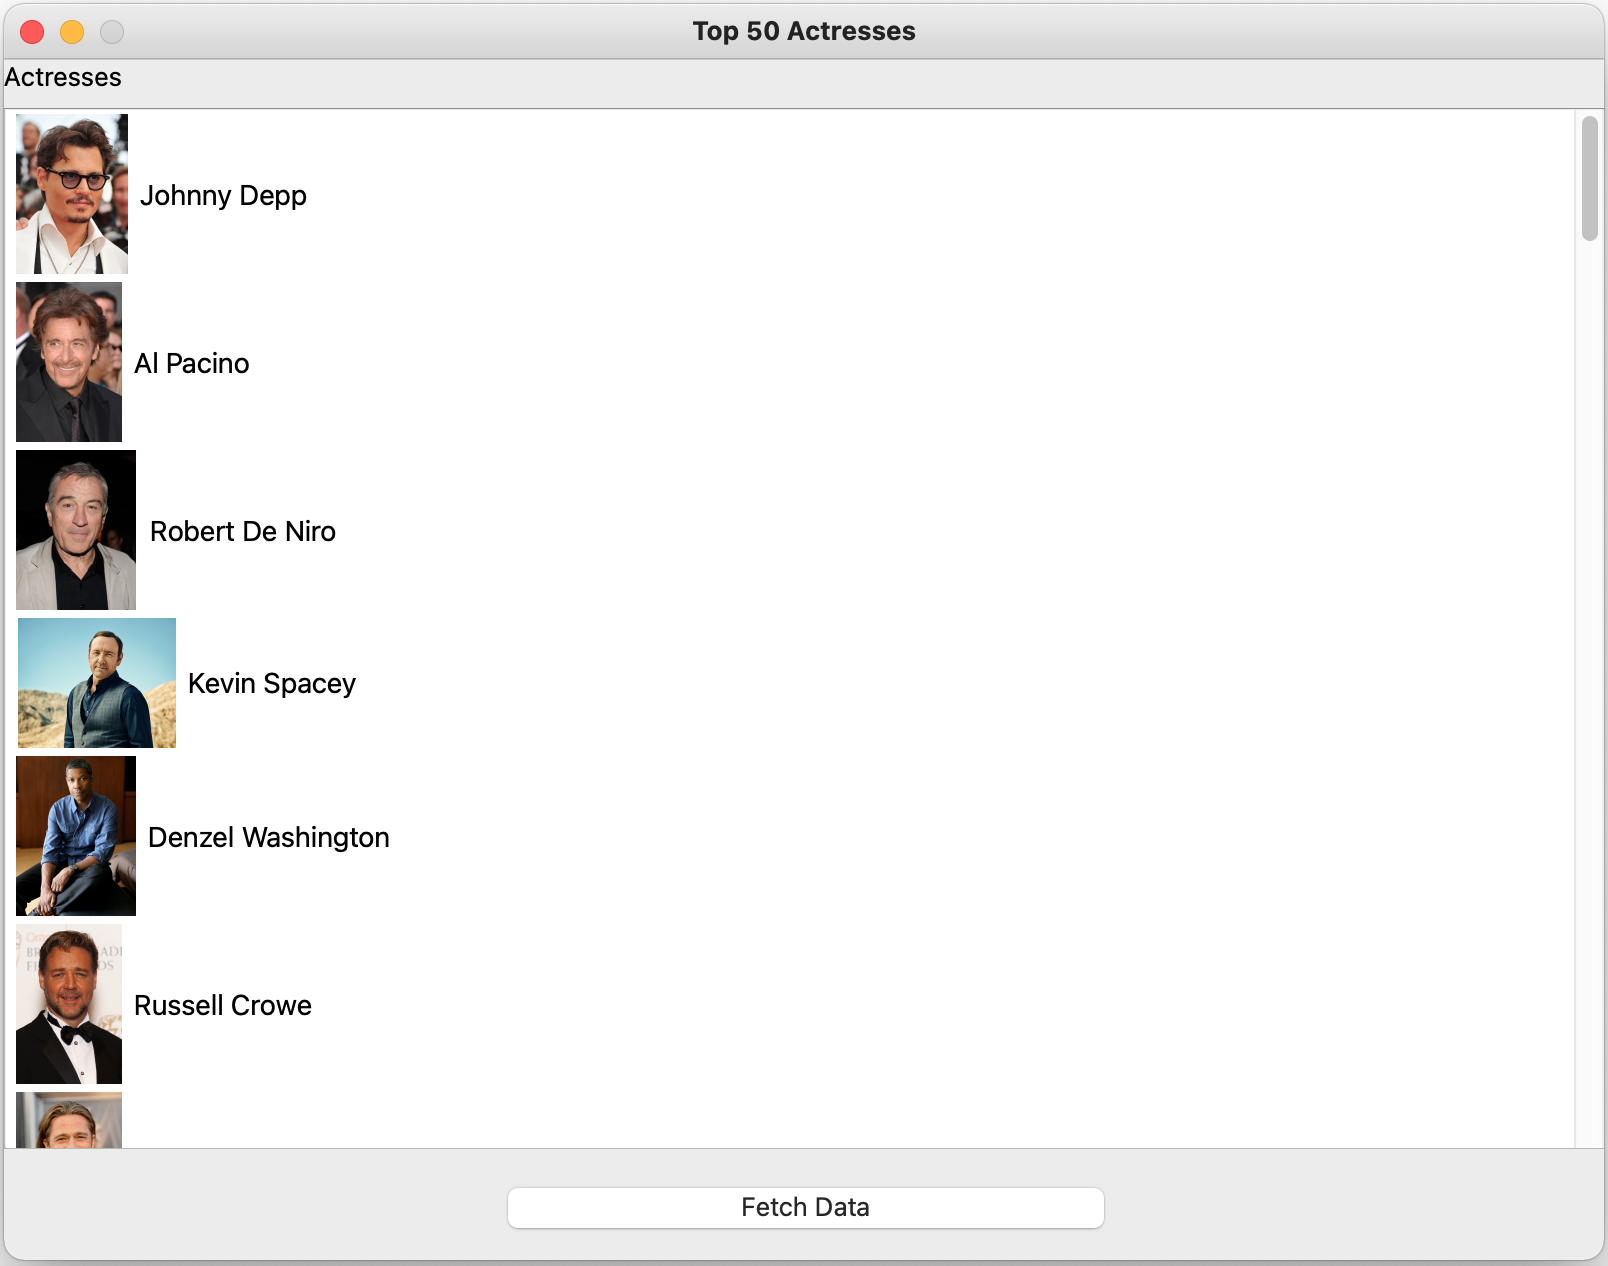
\includegraphics[width=0.45\textwidth]{img/main-window-screen.png}
      \caption[width=0.45\textwidth]{\label{fig:main-window-screen} screenshot of the MainView}
\end{figure}

When the user clicks on the \textit{Fetch Button} the sequence \ref{fig:fetch-actresses-flow} starts
and everytime a new actor/actress is published in actresses list the the actresses table view gets 
updated so the user sees the update process. Here the \textit{IMDB-Api} is used. The extracted JSON file gets translated into a dataframe. Since the fetching is executed in a seperate thread, the 
main thread is not blocked and the UI is responsive. At any time the user can click on the list element
to transition to DetailView of the actress.

\textbf{Main methods:} 
\begin{itemize}
      \item \textit{fetchActressesDataFromUrl(self)}
      \item \textit{fetchActress(self)}
\end{itemize}


\subsection{About the actor/actresses} \label{about}
With a new API call to the actress list of the clicked actress/actor in the MainView 
a new dataframe with Pandas gets created. A short summary for each actor/actress is provided and
therfore used in a textfield. You can see the result in the upper left area of 
fig \ref{fig:detail-window-screen}.

\textbf{Main methods:}
\begin{itemize}
      \item initContent(self, pixmap, name, id)
\end{itemize}

\begin{figure}[h]
      \centering
      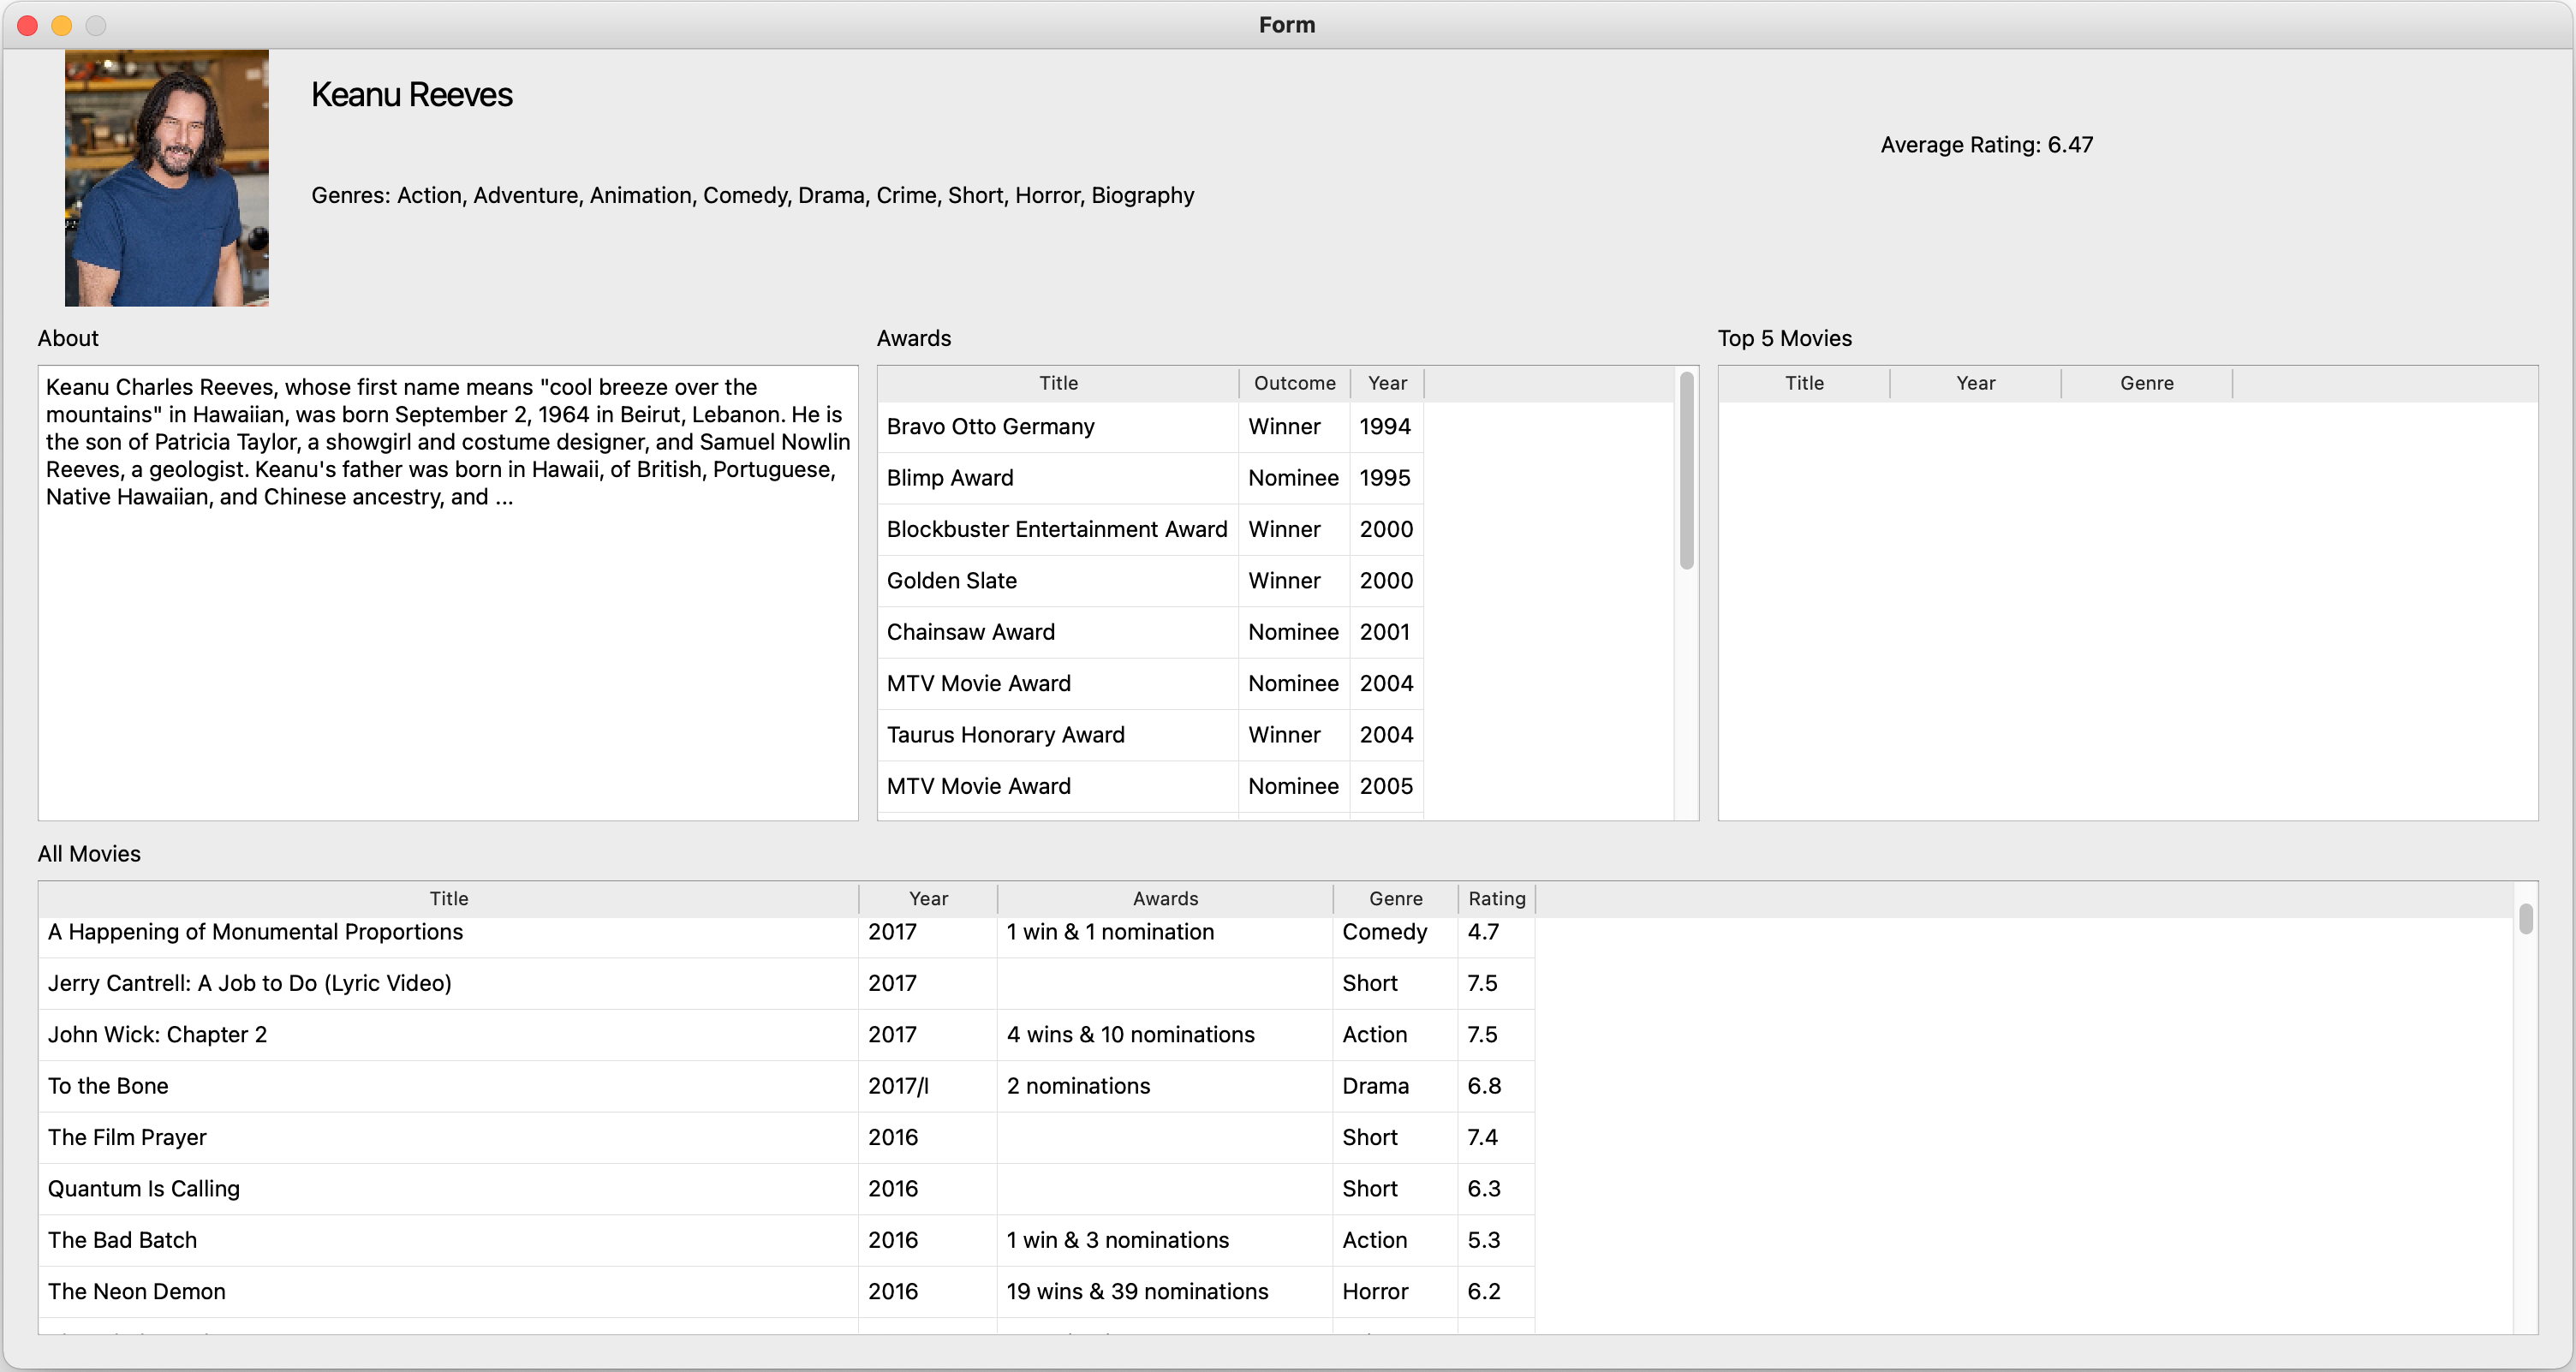
\includegraphics[width=0.7\textwidth]{img/detail-window-screen.png}
      \caption{\label{fig:detail-window-screen} screenshot of the DetailView}
\end{figure}

\subsection{All time movie names and years} \label{movies}
The API call of \ref{about} is also used to gather all movies and their release years of
the provided dataframe. To fill the movies table in the bottom of fig \ref{fig:detail-window-screen} the dataframe gets iterated using the iterrows property of the
dataframe. To display every item correctly, the columns get updated for every insert.

\textbf{Main methods:}
\begin{itemize}
      \item \textit{initContent(self, pixmap, name, id)}
\end{itemize}

\subsection{Awards to actor/actresses in different years} \label{awards}
As the DetailView is presented the ActressAwardDataWorker is triggered for 
execution attached to a seperate thread. 

\begin{figure}[h]
      \centering
      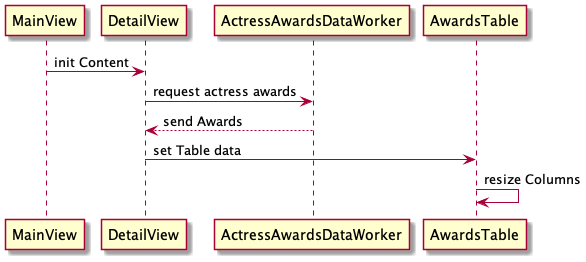
\includegraphics[width=0.7\textwidth]{img/actress-awardsdata-worker-sequence.png}
      \caption{\label{fig:awardsdata-worker-sequence} flowchart of AwardsDataWorker}
\end{figure}

The worker fetches the awards url
of an actor and uses BeautifulSoup to extract a list of awards with the 
outcome (Nominee or Winner) and also the respective year. By iterating over 
the list the awards table get filled (fig \ref{fig:awardsdata-worker-sequence}).

\textbf{Main methods:}
\begin{itemize}
      \item \textit{fetchAwardsData(self)}
\end{itemize}

\subsection{Movie genre of actor/actresses} \label{genre}
\begin{figure}[H]
      \centering
      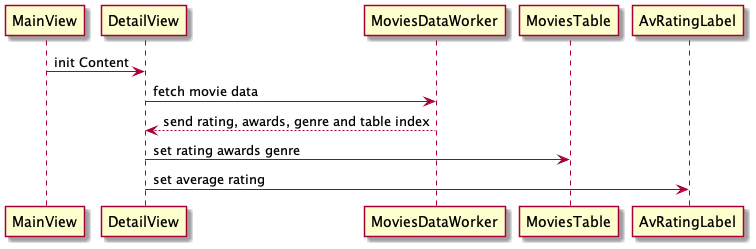
\includegraphics[width=0.8\textwidth]{img/movies-data-worker-sequence.png}
      \caption{\label{fig:movies-data-worker-sequence} flowchart of MoviesDataWorker}
\end{figure}

The worker MoviesDataWorker also gets attached to a thread. After the movies table 
is filled with all the movies. The worker iterates over every movie element in the 
actress movie dataframe and uses the id to fetch the movie site with BeautifulSoup (fig. \ref{fig:movies-data-worker-sequence})

\textbf{Main methods:}
\begin{itemize}
      \item \textit{fetchMovieData(self)}
\end{itemize}

\subsection{Average rating of their movies} \label{average-rating}
While the iteration in \ref{genre} happens everytime when a rating value for the movie exists
a counter gets incremented and the rating is added to an overall rating. The average rating of all
the movies is created and the UI is updated every iteration.

\textbf{Main methods:}
\begin{itemize}
      \item \textit{fetchMovieData(self)}
\end{itemize}

\subsection{Top 5 movies, their respective years and genre} \label{top-movies}
After the MoviesDataWorker (fig. \ref{fig:awardsdata-worker-sequence}) is finished it sends a
signal and the \textit{setTop5Movies} method gets called. To get the top 5 elements Pandas methods
\textit{sort\_values} for sorting and then \textit{head} is used. Now the table for top movies can
easily be filled.

\textbf{Main methods:}
\begin{itemize}
      \item \textit{setTop5Movies(self)}
\end{itemize}

\end{document}
